\documentclass[conference]{IEEEtran}

% Paquetes necesarios
\usepackage[spanish]{babel}
\usepackage{amsmath,amssymb,amsfonts,amsthm}
\usepackage{graphicx}
\usepackage[utf8]{inputenc}
\usepackage{url}
\usepackage{hyperref}
\usepackage{subfig}
\usepackage{balance}
\usepackage{csquotes}
\usepackage{float} % Para controlar la posición de las imágenes
\usepackage[backend=biber, style=ieee]{biblatex} % Paquete de bibliografía
\addbibresource{referencias.bib} % Archivo de bibliografía
\usepackage[parfill]{parskip} % Reduce el espacio entre párrafos
\usepackage{setspace} % Para controlar el espaciado

% Configurar el espacio entre párrafos y líneas
\usepackage[parfill]{parskip}
\setlength{\parskip}{0em} % Configura espacio entre párrafos a 0
\setlength{\parindent}{0em} % Configura sin sangría


%%%%%%%%%%%%%%%%%%%%%%%%%%%%%%%%%%%%%%%%%%%%%
% PARCHE PARA ELIMINAR LA FECHA DEL DOCUMENTO
\usepackage{etoolbox}
\makeatletter
\patchcmd{\frontmatter@RRAP@format}{(}{}{}{}
\patchcmd{\frontmatter@RRAP@format}{)}{}{}{}
\makeatother

\begin{document}

\title{Reporte de Proyecto en Equipo U3 \\ Visualización de un cubo rubik en un plano 2d}

\author{\IEEEauthorblockN{
Ledezma Donjuan Daniel Armando \IEEEauthorrefmark{1}, 
Garcia Gonzalez Allison Esli\IEEEauthorrefmark{1}, \\ Rodriguez Salas Luisana Guadalupe\IEEEauthorrefmark{1}, Olivares Rodriguez Brayan \IEEEauthorrefmark{1} \\ y Rodriguez Chavez Ana Cecilia\IEEEauthorrefmark{1}}
\IEEEauthorblockA{\IEEEauthorrefmark{1}Ingeniería en Tecnologías de la Información\\
Universidad Politécnica de Victoria\\
Victoria, Tamaulipas, México}
}

\maketitle

\begin{abstract}
La aplicación móvil desarrollada busca simplificar la resolución del cubo Rubik mediante un enfoque más accesible. Tradicionalmente, estas simulaciones utilizan entornos 3D, pero este proyecto propone una interfaz en formato horizontal que visualiza un plano 2D del cubo haciendo uso de un diagrama de Venn interactivo, eliminando la necesidad de visualizar todas las caras simultáneamente.

La aplicación se divide en tres secciones: a la derecha, el cubo en 3D; a la izquierda, el plano 2d para controlar movimientos; y en la parte inferior, 18 botones clasificados en movimientos normales e inversos. Este diseño facilita la interacción del usuario, ofreciendo una experiencia más intuitiva y accesible para resolver el cubo Rubik.
\end{abstract}


\section{Introducción}
La resolución del cubo Rubik es un desafío mental popular que pone a prueba la agilidad cognitiva, la memoria espacial y las habilidades para resolver problemas.\cite{bellavista_cubo} A lo largo de los años, se han desarrollado diversas herramientas y métodos para ayudar a los usuarios a aprender a resolver el cubo, incluso sin tenerlo físicamente presente. En este contexto, la aplicación móvil que simula un cubo Rubik fue diseñada con el propósito de ofrecer una alternativa digital para aquellos interesados en resolver el cubo sin la necesidad del objeto físico.

Aunque el propósito exacto de la aplicación original no está claramente definido, se puede inferir que su objetivo era proporcionar a los usuarios una herramienta para resolver el cubo Rubik en un entorno virtual\cite{androiddevelopers_drawables}. Inicialmente, la app permitía manipular el cubo en un espacio tridimensional, lo que brindaba una experiencia de resolución similar a la de un cubo físico, pero sin la necesidad de un objeto tangible.\cite{9gag_rubik}

Con el fin de mejorar la experiencia del usuario y hacer la resolución del cubo más accesible, se decidió integrar un diagrama de Venn interactivo en la aplicación. \cite{canela2019aspectos}Este diagrama no solo facilita la comprensión de cómo resolver el cubo, sino que también ofrece una manera visual de abordar el problema sin la necesidad de ver todas las caras del cubo simultáneamente.\cite{rodriguez2023ejemplos} El plano 2d es completamente interactivo, mostrando los cambios en tiempo real a medida que el usuario interactúa con los botones\cite{edrawsoft_venn}. Los movimientos en el plano 2d se reflejan inmediatamente en el cubo Rubik, ya que ambos están conectados.\cite{androiddevelopers_opengl} Esta integración facilita la resolución del cubo sin la necesidad de ver todas las caras del mismo, haciendo que el proceso sea más sencillo y accesible.\cite{spinelli2005diagrama}

El objetivo principal de este proyecto fue facilitar la resolución del cubo Rubik, mejorando la interacción del usuario mediante una interfaz más accesible y comprensible. Para lograrlo, se implementaron 18 botones que permiten mover el cubo y el plano 2d de manera sincronizada\cite{kessenich2006opengl}. Esta nueva funcionalidad proporciona una manera más sencilla de interactuar con el cubo y permite resolverlo de forma más eficiente.

Este informe describe el proceso de implementación de estas nuevas funcionalidades, los cambios realizados en la aplicación y cómo estos contribuyen a mejorar la experiencia general del usuario al resolver el cubo Rubik.\cite{soriano2019android}


\section{Desarrollo Experimental}

\subsection{Configuración Base} 
El uso de Canvas y OpenGL permitió crear una representación híbrida de un cubo Rubik con características tanto bidimensionales como tridimensionales, mejorando la interacción del usuario y aprovechando las capacidades gráficas de Android.

\begin{itemize}
    \item \textbf{Canvas} se utilizó para la parte bidimensional, específicamente para dibujar el diagrama de Venn, permitiendo controlar directamente el trazado de los círculos y los colores. Esta elección se debió a que Canvas permite manipular gráficos 2D de manera simple y efectiva, lo cual es ideal para representar la intersección de áreas y sus relaciones, proporcionando un nivel de detalle adecuado para esta aplicación.
    
    \item \textbf{OpenGL} se utilizó para la representación tridimensional del cubo Rubik. La capacidad de OpenGL para manejar gráficos 3D en tiempo real fue clave para proporcionar una experiencia visual fluida e interactiva del cubo Rubik. Además, se aprovechó la aceleración por hardware de OpenGL para mejorar el rendimiento de la aplicación en dispositivos móviles. 
\end{itemize}

\subsection{Configuración Específica del Proyecto} 

\begin{itemize}
    \item AndroidManifest.xml: Este archivo contiene la configuración esencial para definir el entorno en el que la aplicación opera. Se incluyeron permisos para internet y para el acceso a recursos gráficos. Aunque en este proyecto no se requería acceso a la ubicación, la preparación de la infraestructura para servicios en línea (como futuras integraciones para compartir estadísticas de resolución o para ofrecer guías interactivas en línea).
    \item build.gradle: En el archivo build.gradle, se definieron dependencias necesarias para manejar las gráficas y la interfaz de usuario, incluyendo bibliotecas para facilitar el renderizado OpenGL y las interacciones mediante gestos. Esto incluyó dependencias para androidx.appcompat para asegurar la compatibilidad y com.google.android.material para proporcionar botones que ofrecieran una experiencia de usuario consistente.
    
\end{itemize}

\subsection{Diseño de Interfaz} 

La interfaz del proyecto fue diseñada con la simplicidad y la claridad como principios fundamentales, permitiendo que el usuario pueda interactuar intuitivamente tanto con el cubo Rubik como con el plano 2d. Este diseño consistió en dividir la pantalla en tres secciones, manteniendo siempre visible la información esencial para resolver el cubo.\newline
Esto se logro primero que nada colocando los botones que ejecutarian los movimientos tanto del cubo como de los nodos en el plano 2d, despues para lograr la vista del plano 2d se implemento un diagrama de venn el cual fue dibujado usando un trangulo equilatero para de esta manera usar sus vertices como epicentros de las 3 secciones de 3 circulos que usariamos, esto debido a que si se dibujaba usando solo coordenadas el diagrama tendia a desacomodarse en distintos dispositivos debido a que tomaba como base que la pantalla siempre seria de 1080 px y por esto afectaba a otros dispositivos que no tenian esta resolucion. Y los nodos que actuaban como visualizacion para las caras del cubo rubik se colocan en 6 secciones de 9 nodos debido a que asi estan distribuidas las caras del cubo rubik. Estos nodos se colocan en los vertices formados por el diagrama de venn haciendo asi que simule de manera precisa los movimientos de un cubo rubik.

\subsubsection{Distribución y Layout de la Pantalla} 

\begin{itemize}
    \item Parte Izquierda (plano 2d): En la sección izquierda de la pantalla se encuentra el plano 2d, que representa tres caras del cubo Rubik. Este diagrama está compuesto por tres grupos de círculos concéntricos que se intersectan, y cada uno de estos grupos contiene nueve nodos, los cuales representan una de las caras del cubo Rubik. Cada nodo simboliza un "cubo" individual de la cara, de manera que se puede visualizar cómo los movimientos afectan a diferentes partes del cubo. Los nodos se encuentran organizados en grupos de 3x3, y cada nodo dentro de estos grupos refleja el estado de uno de los cubos pequeños (subcubos) que componen la cara del cubo Rubik. Al realizar movimientos, el usuario puede observar cómo los colores se desplazan entre los nodos, lo cual visualiza los giros y su impacto sobre las tres caras principales que son visibles en el diagrama.
    \item Parte Derecha (Cubo Rubik): En el lado derecho de la pantalla se encuentra la vista tridimensional del cubo Rubik, renderizada mediante VistaCubo utilizando OpenGL. La elección de situar el cubo a la derecha se debe a que esta disposición refleja un flujo de trabajo natural para usuarios diestros, quienes tienden a mirar primero a la izquierda para comprender el contexto (plano 2d) y luego a la derecha para ejecutar acciones o verificar resultados.
    \item Parte Inferior (Controles de Movimiento): La parte inferior contiene los botones de control. Hay un total de 18 botones que representan movimientos básicos (L, R, F, etc.) y movimientos de las capas medias (M, E, S). Los botones se diseñaron con la biblioteca de Material Design (MaterialButton), lo que asegura que el diseño sea consistente y que los botones sean fáciles de identificar y presionar. La separación entre movimientos con y sin ' (prima) facilita que los usuarios diferencien entre rotaciones. \newline
\end{itemize} 

\subsection{Lógica de Movimiento del Cubo Rubik} 
La implementación de la lógica de movimiento del cubo Rubik se realizó principalmente mediante la clase CubeMovementHandler, la cual se encarga de procesar los movimientos solicitados por el usuario y de sincronizarlos entre la representación gráfica (VistaCubo) y el modelo de datos interno.

A continuación, se presenta un seudocódigo que describe el flujo general de la aplicación y cómo los diferentes componentes interactúan entre sí:

\begin{verbatim}
\small
Inicio de la aplicación MainActivity:
1. Configurar pantalla completa sin título.
2. Establecer el diseño principal 
desde el archivo XML.
3. Inicializar el componente
VennDiagramView desde el layout.
4. Crear una instancia de VistaCubo 
y añadirla al contenedor derecho (si existe).

Configuración de los botones:
5. Para cada botón (L, L', F, F', etc.):
   a. Asociar un movimiento 
   y una acción en VennDiagramView al botón.
   b. Configurar el botón para ejecutar:
    i. Un movimiento en VistaCubo.
    ii. Una acción correspondiente
    en VennDiagramView.

Acción al presionar un botón:
6. Al presionar un botón:
   a. Ejecutar el movimiento en VistaCubo.
   b. Ejecutar la acción en VennDiagramView.

Procesar movimientos del cubo:
7. Determinar el tipo de movimiento 
(cara, línea y sentido).
8. Girar visualmente la cara del cubo.
9. Actualizar la estructura interna
de datos del cubo.

Métodos del ciclo de vida:
10. En reanudar la actividad 
(onResume), reanudar VistaCubo.
11. En pausar la actividad (onPause),
pausar VistaCubo.
\end{verbatim}

Este flujo permite asegurar que cada acción tomada por el usuario en la interfaz se refleje correctamente tanto en la vista del cubo Rubik como en el plano 2D.

\subsubsection{Implementación Modular de Movimientos} 
\begin{itemize}
    \item Método handleMove(): Cada vez que el usuario presiona un botón, el método handleMove(String move) de CubeMovementHandler toma el movimiento y lo coloca en la cola de eventos de OpenGL (vistaCubo.queueEvent()). Este enfoque permite que los movimientos sean procesados de forma asíncrona, evitando el bloqueo del hilo principal de la aplicación y mejorando la fluidez del movimiento.
    \item Método processMove(): El método processMove(String move) determina si el movimiento debe ser en sentido horario o antihorario. Se verifica si el movimiento contiene un símbolo ' (prima) para determinar la dirección. Dependiendo del movimiento (por ejemplo, L, R, F, etc.), el método llama a rotateFace() para aplicar la rotación en la cara o capa correspondiente del cubo.
    \item Método rotateFace(): Este método aplica el ángulo de rotación (90° o -90°) a una cara específica del cubo Rubik, primero actualizando la representación visual (girarReferenciasGL) y luego actualizando la estructura interna (girarReferencias). Se implementó un breve retardo (Thread.sleep(50)) para asegurar que la rotación fuera visualmente suave, evitando movimientos abruptos que pudieran generar confusión en el usuario.
\end{itemize}

\subsection{Sincronización de Nodos del Diagrama y Movimientos del Cubo} 

Cada nodo dentro del plano 2d representa un subcubo específico de una cara del cubo Rubik. Esto quiere decir que cada cara visible en el plano 2d está dividida en 9 nodos que corresponden a los 9 subcubos que forman una cara del cubo Rubik completo.

\begin{itemize}
    \item Nodos como Subcubos: Los nodos se actualizan cada vez que el usuario realiza un movimiento, y este desplazamiento de colores entre los nodos ayuda a comprender cómo los giros del cubo Rubik afectan las tres caras representadas por el plano 2d. Cada sección de 9 nodos actúa como una representación simplificada de una de las caras del cubo Rubik, lo que significa que cada nodo individual muestra el estado de uno de los subcubos.
    \item Interactividad de los Nodos: Los movimientos de los nodos se gestionan mediante la clase VennDiagramView, que tiene métodos específicos para desplazar los colores y actualizar la vista de los nodos. Estos métodos (shiftColors(), setupBlocks(), etc.) se encargan de sincronizar los cambios de estado de cada nodo con los movimientos realizados sobre el cubo Rubik en VistaCubo. Cada vez que el usuario presiona un botón, se desencadena un movimiento tanto en la vista tridimensional como en los nodos del plano 2d, ofreciendo una retroalimentación visual clara y efectiva (VennDiagramView).
  
\end{itemize}

\subsection{Sincronización entre Vistas: Cubo Rubik y plano 2d} 

Uno de los desafíos clave del proyecto fue lograr la sincronización entre el cubo Rubik y el plano 2d para asegurar que cualquier movimiento realizado por el usuario se refleje correctamente en ambas vistas. Para esto, se utilizaron varias estrategias:

\begin{itemize}
    \item Actualización en Tiempo Real de Nodos y Movimientos: Para mantener la sincronización entre los nodos del plano 2d y las caras del cubo Rubik, cada vez que se realiza un movimiento, se ejecutan acciones tanto en la vista del cubo como en el diagrama. Los nodos reflejan instantáneamente el estado actualizado de las caras afectadas, proporcionando una representación visual que es fácil de seguir.
    \item Control de Sincronización mediante MainActivity: La clase MainActivity configura los botones de la interfaz para que, cuando el usuario presione un botón, el movimiento del cubo Rubik se ejecute al mismo tiempo que se actualizan los nodos correspondientes en el plano 2d. Esta sincronización asegura que el usuario vea cómo los movimientos afectan a los diferentes nodos, permitiéndoles comprender mejor las relaciones entre los giros del cubo y el estado final (MainActivity).
\end{itemize}

\section{Resultados}
La aplicación desarrollada logró cumplir los objetivos planteados al integrar de manera efectiva la representación visual de un cubo Rubik en un plano en 2d, sincronizados en tiempo real. Los movimientos realizados en el cubo tridimensional se reflejan inmediatamente en el plano, lo que permite al usuario observar cómo los giros afectan las diferentes caras de manera clara y visualmente accesible. Este diseño resultó en una experiencia de usuario fluida, donde tanto los principiantes como los usuarios experimentados pueden comprender los estados intermedios del cubo con mayor facilidad.

En su estado inicial, la aplicación permite observar el cubo Rubik completamente armado junto con su correspondiente representación gráfica en el plano 2d, reflejando las caras en una configuración resuelta. Al realizar un solo movimiento, como girar la cara izquierda (L) como se muestra en la figura \ref{fig:cambio al girar}, los cambios se evidencian tanto en la visualización tridimensional del cubo como en el plano 2d, mostrando cómo dicho giro afecta la disposición de los colores en las intersecciones del grafo. A medida que se realizan más movimientos en el cubo, se observa cómo ambas representaciones se vuelven más desordenadas; esto se logra ver en la figura \ref{fig:Desordenadas}, lo que refleja con precisión la complejidad y el desafío de resolver el cubo.

\subsection{Interfaz Principal}
La interfaz de usuario se diseñó considerando una experiencia fluida e intuitiva, como se muestra a continuación en la figura \ref{fig:cubo Rubik}:

\begin{itemize}
    \item \textbf{Parte Izquierda (plano 2d)}:En la parte izquierda se muestra el plano 2d, que representa tres caras del cubo Rubik con círculos concéntricos y nodos 3x3. Los colores de los nodos cambian al ejecutar movimientos, visualizando cómo los giros afectan las tres caras principales del cubo.
    \item \textbf{Parte Derecha (Cubo Rubik)}: En el lado derecho de la pantalla se muestra la vista tridimensional del cubo Rubik, renderizada mediante la clase VistaCubo utilizando OpenGL.
    \item \textbf{Parte Inferior (Controles de Movimiento)}: En la parte inferior se encuentran 18 botones de control, diseñados con Material Design, que representan movimientos básicos y de las capas medias. La distinción entre movimientos con y sin prima ) permite diferenciar entre rotaciones.
\end{itemize} 

\begin{figure}[H]
    \centering
    \includegraphics[width=1\linewidth]{b.jpeg} 
    \caption{\textbf{Cambio al girar una cara (L):} Aquí se visualiza cómo un giro en la cara izquierda del cubo Rubik altera tanto su configuración tridimensional como las intersecciones del diagrama de Venn, reflejando de manera precisa el movimiento realizado.}
    \label{fig:cambio al girar}
\end{figure}

\begin{figure}[H]
    \centering
    \includegraphics[width=1\linewidth]{c.jpeg} 
    \caption{\textbf{Estado desordenado tras múltiples movimientos:} En esta imagen se presenta el cubo Rubik después de realizar varios giros, con una disposición caótica de colores que también se refleja en el diagrama de Venn, mostrando cómo las caras y sus intersecciones se ven afectadas en el proceso.}
    \label{fig:Desordenadas}
\end{figure}

\begin{figure}[H]
    \centering
    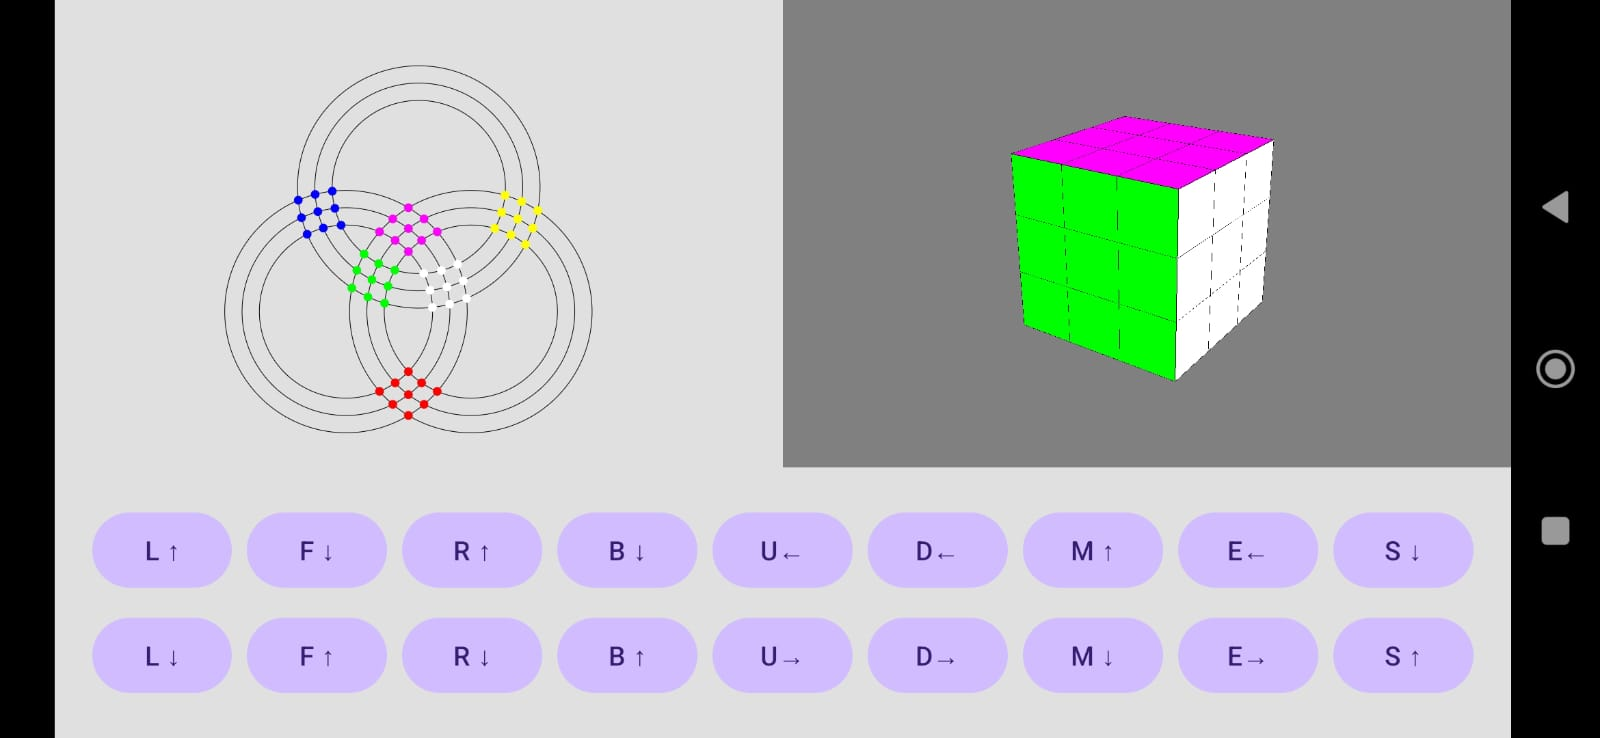
\includegraphics[width=1\linewidth]{a.jpeg} 
    \caption{\textbf{Interfaz, Cubo Rubik y diagrama inicial completamente armados:} En esta imagen se muestra el estado resuelto del cubo Rubik y su representación en el diagrama de Venn, donde los colores están organizados y las caras perfectamente alineadas.}
    \label{fig:cubo Rubik}
\end{figure}

\section{Conclusión}
En este proyecto se desarrolló una aplicación móvil orientada a simplificar la resolución del cubo Rubik, integrando un diseño innovador que combina un plano 2D del cubo con un diagrama de Venn interactivo. Esta propuesta representa una alternativa accesible frente a los entornos tridimensionales tradicionales, reduciendo la complejidad visual y mejorando la experiencia del usuario.

Los resultados obtenidos destacan la sincronización efectiva entre el cubo y el diagrama, permitiendo movimientos en tiempo real mediante botones intuitivos que clasifican las rotaciones normales e inversas. La aplicación demostró ser una herramienta eficiente para aprender y practicar la resolución del cubo Rubik.

Sin embargo, la solución presenta ciertas limitaciones, como la falta de opciones personalizables para niveles avanzados. Futuras mejoras podrían incluir tutoriales interactivos, estadísticas de resolución y sincronización en la nube para compartir progresos entre dispositivos. Con estas adiciones, se podría extender aún más el alcance y utilidad de la aplicación.

\printbibliography

\end{document}